%\documentclass{standalone}
%\documentclass[a4paper,class=article,border=0pt]{standalone}
\documentclass[tikz,margin=0.5pt]{standalone}
\usepackage{tikz}
\usepackage{pdftricks}
\begin{psinputs}
  \usepackage{pstricks}
  \usepackage{pst-node}
\end{psinputs}
%\documentclass{article}
%\documentclass[margin=3pt,pdftricks]{standalone}
%\begin{psinputs}
  %\usepackage{pstricks}
  %\usepackage{pst-node}
%\end{psinputs}
\usepackage{pgfplots}
\usepackage{xparse}
\usepackage{graphicx}
\usetikzlibrary{shapes,arrows,positioning}
\usepackage{xspace,amsmath}

\def\Palpha      {\ensuremath{\alpha}\xspace}
\def\Pbeta       {\ensuremath{\beta}\xspace}
\def\Pgamma      {\ensuremath{\gamma}\xspace}
\def\Pdelta      {\ensuremath{\delta}\xspace}
\def\Pepsilon    {\ensuremath{\epsilon}\xspace}
\def\Pvarepsilon {\ensuremath{\varepsilon}\xspace}
\def\Pzeta       {\ensuremath{\zeta}\xspace}
\def\Peta        {\ensuremath{\eta}\xspace}
\def\Ptheta      {\ensuremath{\theta}\xspace}
\def\Pvartheta   {\ensuremath{\vartheta}\xspace}
\def\Piota       {\ensuremath{\iota}\xspace}
\def\Pkappa      {\ensuremath{\kappa}\xspace}
\def\Plambda     {\ensuremath{\lambda}\xspace}
\def\Pmu         {\ensuremath{\mu}\xspace}
\def\Pnu         {\ensuremath{\nu}\xspace}
\def\Pxi         {\ensuremath{\xi}\xspace}
\def\Ppi         {\ensuremath{\pi}\xspace}
\def\Pvarpi      {\ensuremath{\varpi}\xspace}
\def\Prho        {\ensuremath{\rho}\xspace}
\def\Pvarrho     {\ensuremath{\varrho}\xspace}
\def\Ptau        {\ensuremath{\tau}\xspace}
\def\Pupsilon    {\ensuremath{\upsilon}\xspace}
\def\Pphi        {\ensuremath{\phi}\xspace}
\def\Pvarphi     {\ensuremath{\varphi}\xspace}
\def\Pchi        {\ensuremath{\chi}\xspace}
\def\Ppsi        {\ensuremath{\psi}\xspace}
\def\Pomega      {\ensuremath{\omega}\xspace}
\mathchardef\PDelta="7101
\mathchardef\PXi="7104
\mathchardef\PLambda="7103
\mathchardef\PSigma="7106
\mathchardef\POmega="710A
\mathchardef\PUpsilon="7107
\def\PA      {\ensuremath{A}\xspace}
\def\PB      {\ensuremath{B}\xspace}
\def\PC      {\ensuremath{C}\xspace}
\def\PD      {\ensuremath{D}\xspace}
\def\PE      {\ensuremath{E}\xspace}
\def\PF      {\ensuremath{F}\xspace}
\def\PG      {\ensuremath{G}\xspace}
\def\PH      {\ensuremath{H}\xspace}
\def\PI      {\ensuremath{I}\xspace}
\def\PJ      {\ensuremath{J}\xspace}
\def\PK      {\ensuremath{K}\xspace}
\def\PL      {\ensuremath{L}\xspace}
\def\PM      {\ensuremath{M}\xspace}
\def\PN      {\ensuremath{N}\xspace}
\def\PO      {\ensuremath{O}\xspace}
\def\PP      {\ensuremath{P}\xspace}
\def\PQ      {\ensuremath{Q}\xspace}
\def\PR      {\ensuremath{R}\xspace}
\def\PS      {\ensuremath{S}\xspace}
\def\PT      {\ensuremath{T}\xspace}
\def\PU      {\ensuremath{U}\xspace}
\def\PV      {\ensuremath{V}\xspace}
\def\PW      {\ensuremath{W}\xspace}
\def\PX      {\ensuremath{X}\xspace}
\def\PY      {\ensuremath{Y}\xspace}
\def\PZ      {\ensuremath{Z}\xspace}
\def\Pa      {\ensuremath{a}\xspace}
\def\Pb      {\ensuremath{b}\xspace}
\def\Pc      {\ensuremath{c}\xspace}
\def\Pd      {\ensuremath{d}\xspace}
\def\Pe      {\ensuremath{e}\xspace}
\def\Pf      {\ensuremath{f}\xspace}
\def\Pg      {\ensuremath{g}\xspace}
\def\Ph      {\ensuremath{h}\xspace}
\def\Pi      {\ensuremath{i}\xspace}
\def\Pj      {\ensuremath{j}\xspace}
\def\Pk      {\ensuremath{k}\xspace}
\def\Pl      {\ensuremath{l}\xspace}
\def\Pm      {\ensuremath{m}\xspace}
\def\Pn      {\ensuremath{n}\xspace}
\def\Po      {\ensuremath{o}\xspace}
\def\Pp      {\ensuremath{p}\xspace}
\def\Pq      {\ensuremath{q}\xspace}
\def\Pr      {\ensuremath{r}\xspace}
\def\Ps      {\ensuremath{s}\xspace}
\def\Pt      {\ensuremath{t}\xspace}
\def\Pu      {\ensuremath{u}\xspace}
\def\Pv      {\ensuremath{v}\xspace}
\def\Pw      {\ensuremath{w}\xspace}
\def\Px      {\ensuremath{x}\xspace}
\def\Py      {\ensuremath{y}\xspace}
\def\Pz      {\ensuremath{z}\xspace}





%%%%%%%%%%%%%%%%%%%%%%%%%%%%%%%%%%%%%%%%%%%%%%%
% Particles

%% Leptons

\let\emi\en
\def\electron   {\ensuremath{\Pe}\xspace}
\def\en         {\ensuremath{\Pe^-}\xspace}   % electron negative (\em is taken)
\def\ep         {\ensuremath{\Pe^+}\xspace}
\def\epm        {\ensuremath{\Pe^\pm}\xspace}
\def\epem       {\ensuremath{\Pe^+\Pe^-}\xspace}
\def\ee         {\ensuremath{\Pe^-\Pe^-}\xspace}

\def\mmu        {\ensuremath{\Pmu}\xspace}
\def\mup        {\ensuremath{\Pmu^+}\xspace}
\def\mun        {\ensuremath{\Pmu^-}\xspace} % muon negative (\mum is taken)
\def\mumu       {\ensuremath{\Pmu^+\Pmu^-}\xspace}
\def\mtau       {\ensuremath{\Ptau}\xspace}

\def\taup       {\ensuremath{\Ptau^+}\xspace}
\def\taum       {\ensuremath{\Ptau^-}\xspace}
\def\tautau     {\ensuremath{\Ptau^+\Ptau^-}\xspace}

\def\ellm       {\ensuremath{\ell^-}\xspace}
\def\ellp       {\ensuremath{\ell^+}\xspace}
\def\ellell     {\ensuremath{\ell^+ \ell^-}\xspace}

\def\neu        {\ensuremath{\Pnu}\xspace}
\def\neub       {\ensuremath{\overline{\Pnu}}\xspace}
\def\nuenueb    {\ensuremath{\neu\neub}\xspace}
\def\neue       {\ensuremath{\neu_e}\xspace}
\def\neueb      {\ensuremath{\neub_e}\xspace}
\def\neueneueb  {\ensuremath{\neue\neueb}\xspace}
\def\neum       {\ensuremath{\neu_\mu}\xspace}
\def\neumb      {\ensuremath{\neub_\mu}\xspace}
\def\neumneumb  {\ensuremath{\neum\neumb}\xspace}
\def\neut       {\ensuremath{\neu_\tau}\xspace}
\def\neutb      {\ensuremath{\neub_\tau}\xspace}
\def\neutneutb  {\ensuremath{\neut\neutb}\xspace}
\def\neul       {\ensuremath{\neu_\ell}\xspace}
\def\neulb      {\ensuremath{\neub_\ell}\xspace}
\def\neulneulb  {\ensuremath{\neul\neulb}\xspace}

%% Gauge bosons and scalars

\def\g      {\ensuremath{\Pgamma}\xspace}
\def\H      {\ensuremath{\PH^0}\xspace}
\def\Hp     {\ensuremath{\PH^+}\xspace}
\def\Hm     {\ensuremath{\PH^-}\xspace}
\def\Hpm    {\ensuremath{\PH^\pm}\xspace}
\def\W      {\ensuremath{\PW}\xspace}
\def\Wp     {\ensuremath{\PW^+}\xspace}
\def\Wm     {\ensuremath{\PW^-}\xspace}
\def\Wpm    {\ensuremath{\PW^\pm}\xspace}
\def\Z      {\ensuremath{\PZ^0}\xspace}

%% Quarks

\def\quark     {\ensuremath{\Pq}\xspace}
\def\quarkbar  {\ensuremath{\kern 0.2em\overline{\kern-0.2em\quark}\xspace}}
\def\qqbar     {\ensuremath{\quark\quarkbar}\xspace}
\def\uquark    {\ensuremath{\Pu}\xspace}
\def\uquarkbar {\ensuremath{\kern 0.2em\overline{\kern-0.2em\uquark}\xspace}}
\def\uubar     {\ensuremath{\uquark\uquarkbar}\xspace}
\def\dquark    {\ensuremath{\Pd}\xspace}
\def\dquarkbar {\ensuremath{\kern 0.2em\overline{\kern-0.2em\dquark}\xspace}}
\def\ddbar     {\ensuremath{\dquark\dquarkbar}\xspace}
\def\squark    {\ensuremath{\Ps}\xspace}
\def\squarkbar {\ensuremath{\kern 0.2em\overline{\kern-0.2em\squark}\xspace}}
\def\ssbar     {\ensuremath{\squark\squarkbar}\xspace}
\def\cquark    {\ensuremath{\Pc}\xspace}
\def\cquarkbar {\ensuremath{\kern 0.2em\overline{\kern-0.2em\cquark}\xspace}}
\def\ccbar     {\ensuremath{\cquark\cquarkbar}\xspace}
\def\bquark    {\ensuremath{\Pb}\xspace}
\def\bquarkbar {\ensuremath{\kern 0.2em\overline{\kern-0.2em\bquark}\xspace}}
\def\bbbar     {\ensuremath{\bquark\bquarkbar}\xspace}
\def\tquark    {\ensuremath{\Pt}\xspace}
\def\tquarkbar {\ensuremath{\kern 0.2em\overline{\kern-0.2em\tquark}\xspace}}
\def\ttbar     {\ensuremath{\tquark\tquarkbar}\xspace}

%% Light mesons

\def\pion  {\ensuremath{\Ppi}\xspace}
\def\piz   {\ensuremath{\pion^0}\xspace}
\def\pizs  {\ensuremath{\pion^0\mbox\,\rm{s}}\xspace}
\def\ppz   {\ensuremath{\pion^0\pion^0}\xspace}
\def\pip   {\ensuremath{\pion^+}\xspace}
\def\pim   {\ensuremath{\pion^-}\xspace}
\def\pipi  {\ensuremath{\pion^+\pion^-}\xspace}
\def\pipm  {\ensuremath{\pion^\pm}\xspace}
\def\pimp  {\ensuremath{\pion^\mp}\xspace}

\def\kaon  {\ensuremath{\PK}\xspace}
%%% do NOT use ensuremath here
  \def\Kbar  {\kern 0.2em\overline{\kern -0.2em \PK}{}\xspace}
\def\Kb    {\ensuremath{\Kbar}\xspace}
\def\Kz    {\ensuremath{\kaon^0}\xspace}
\def\Kzb   {\ensuremath{\Kbar^0}\xspace}
\def\KzKzb {\ensuremath{\Kz \kern -0.16em \Kzb}\xspace}
\def\Kp    {\ensuremath{\kaon^+}\xspace}
\def\Km    {\ensuremath{\kaon^-}\xspace}
\def\Kpm   {\ensuremath{\kaon^\pm}\xspace}
\def\Kmp   {\ensuremath{\kaon^\mp}\xspace}
\def\KpKm  {\ensuremath{\Kp \kern -0.16em \Km}\xspace}
\def\KS    {\ensuremath{\kaon^0_{\rm\scriptscriptstyle S}}\xspace}
\def\KL    {\ensuremath{\kaon^0_{\rm\scriptscriptstyle L}}\xspace}
\def\Kstarz  {\ensuremath{\kaon^{*0}}\xspace}
\def\Kstarzb {\ensuremath{\Kbar^{*0}}\xspace}
\def\Kstar   {\ensuremath{\kaon^*}\xspace}
\def\Kstarb  {\ensuremath{\Kbar^*}\xspace}
\def\Kstarp  {\ensuremath{\kaon^{*+}}\xspace}
\def\Kstarm  {\ensuremath{\kaon^{*-}}\xspace}
\def\Kstarpm {\ensuremath{\kaon^{*\pm}}\xspace}
\def\Kstarmp {\ensuremath{\kaon^{*\mp}}\xspace}

\newcommand{\etapr}{\ensuremath{\Peta^{\prime}}\xspace}

%% Heavy mesons

%%% do NOT use ensuremath here
  \def\Dbar    {\kern 0.2em\overline{\kern -0.2em \PD}{}\xspace}
\def\D       {\ensuremath{\PD}\xspace}
\def\Db      {\ensuremath{\Dbar}\xspace}
\def\Dz      {\ensuremath{\D^0}\xspace}
\def\Dzb     {\ensuremath{\Dbar^0}\xspace}
\def\DzDzb   {\ensuremath{\Dz {\kern -0.16em \Dzb}}\xspace}
\def\Dp      {\ensuremath{\D^+}\xspace}
\def\Dm      {\ensuremath{\D^-}\xspace}
\def\Dpm     {\ensuremath{\D^\pm}\xspace}
\def\Dmp     {\ensuremath{\D^\mp}\xspace}
\def\DpDm    {\ensuremath{\Dp {\kern -0.16em \Dm}}\xspace}
\def\Dstar   {\ensuremath{\D^*}\xspace}
\def\Dstarb  {\ensuremath{\Dbar^*}\xspace}
\def\Dstarz  {\ensuremath{\D^{*0}}\xspace}
\def\Dstarzb {\ensuremath{\Dbar^{*0}}\xspace}
\def\Dstarp  {\ensuremath{\D^{*+}}\xspace}
\def\Dstarm  {\ensuremath{\D^{*-}}\xspace}
\def\Dstarpm {\ensuremath{\D^{*\pm}}\xspace}
\def\Dstarmp {\ensuremath{\D^{*\mp}}\xspace}
\def\Ds      {\ensuremath{\D^+_\squark}\xspace}
\def\Dsp     {\ensuremath{\D^+_\squark}\xspace}
\def\Dsm     {\ensuremath{\D^-_\squark}\xspace}
\def\Dspm    {\ensuremath{\D^{\pm}_\squark}\xspace}
\def\Dsmp    {\ensuremath{\D^{\mp}_\squark}\xspace}
\def\Dss     {\ensuremath{\D^{*+}_\squark}\xspace}
\def\Dssp    {\ensuremath{\D^{*+}_\squark}\xspace}
\def\Dssm    {\ensuremath{\D^{*-}_\squark}\xspace}
\def\Dsspm   {\ensuremath{\D^{*\pm}_\squark}\xspace}

\def\B       {\ensuremath{\PB}\xspace}
%%% do NOT use ensuremath here
  \def\Bbar    {\kern 0.18em\overline{\kern -0.18em \PB}{}\xspace}
\def\Bb      {\ensuremath{\Bbar}\xspace}
\def\BBbar   {\ensuremath{\B\Bbar}\xspace}
\def\Bz      {\ensuremath{\B^0}\xspace}
\def\Bzb     {\ensuremath{\Bbar^0}\xspace}
\def\Bu      {\ensuremath{\B^+}\xspace}
\def\Bub     {\ensuremath{\B^-}\xspace}
\def\Bp      {\ensuremath{\Bu}\xspace}
\def\Bm      {\ensuremath{\Bub}\xspace}
\def\Bpm     {\ensuremath{\B^\pm}\xspace}
\def\Bmp     {\ensuremath{\B^\mp}\xspace}
\def\Bd      {\ensuremath{\B^0}\xspace}
\def\Bs      {\ensuremath{\B^0_\squark}\xspace}
\def\Bsb     {\ensuremath{\Bbar^0_\squark}\xspace}
\def\Bdb     {\ensuremath{\Bbar^0}\xspace}
\def\Bc      {\ensuremath{\B_\cquark^+}\xspace}
\def\Bcp     {\ensuremath{\B_\cquark^+}\xspace}
\def\Bcm     {\ensuremath{\B_\cquark^-}\xspace}
\def\Bcpm    {\ensuremath{\B_\cquark^\pm}\xspace}

%% Onia

\def\jpsi     {\ensuremath{{\PJ\mskip -3mu/\mskip -2mu\Ppsi\mskip 2mu}}\xspace}
\def\psitwos  {\ensuremath{\Ppsi{(2S)}}\xspace}
\def\psiprpr  {\ensuremath{\Ppsi(3770)}\xspace}
\def\etac     {\ensuremath{\Peta_\cquark}\xspace}
\def\chiczero {\ensuremath{\Pchi_{\cquark 0}}\xspace}
\def\chicone  {\ensuremath{\Pchi_{\cquark 1}}\xspace}
\def\chictwo  {\ensuremath{\Pchi_{\cquark 2}}\xspace}
  %\mathchardef\Upsilon="7107
  \def\Y#1S{\ensuremath{\PUpsilon{(#1S)}}\xspace}% no space before {...}!
\def\OneS  {\Y1S}
\def\TwoS  {\Y2S}
\def\ThreeS{\Y3S}
\def\FourS {\Y4S}
\def\FiveS {\Y5S}

\def\chic  {\ensuremath{\Pchi_{c}}\xspace}

%% Baryons

\def\proton      {\ensuremath{\Pp}\xspace}
\def\antiproton  {\ensuremath{\overline \proton}\xspace}
\def\neutron     {\ensuremath{\Pn}\xspace}
\def\antineutron {\ensuremath{\overline \neutron}\xspace}

\def\Deltares {\ensuremath{\PDelta}\xspace}
\def\Deltaresbar{\ensuremath{\overline \Deltares}\xspace}
\def\Xires {\ensuremath{\PXi}\xspace}
\def\Xiresbar{\ensuremath{\overline \Xires}\xspace}
\def\L {\ensuremath{\PLambda}\xspace}
\def\Lbar {\ensuremath{\kern 0.1em\overline{\kern -0.1em\PLambda}}\xspace}
\def\Lambdares {\ensuremath{\PLambda}\xspace}
\def\Lambdaresbar{\ensuremath{\Lbar}\xspace}
\def\Sigmares {\ensuremath{\PSigma}\xspace}
\def\Sigmaresbar{\ensuremath{\overline \Sigmares}\xspace}
\def\Omegares {\ensuremath{\POmega}\xspace}
\def\Omegaresbar{\ensuremath{\overline \Omegares}\xspace}

%%% do NOT use ensuremath here
 % \def\Deltabar{\kern 0.25em\overline{\kern -0.25em \Deltares}{}\xspace}
 % \def\Sigbar{\kern 0.2em\overline{\kern -0.2em \Sigma}{}\xspace}
 % \def\Xibar{\kern 0.2em\overline{\kern -0.2em \Xi}{}\xspace}
 % \def\Obar{\kern 0.2em\overline{\kern -0.2em \Omega}{}\xspace}
 % \def\Nbar{\kern 0.2em\overline{\kern -0.2em N}{}\xspace}
 % \def\Xb{\kern 0.2em\overline{\kern -0.2em X}{}\xspace}

\def\Lb      {\ensuremath{\L^0_\bquark}\xspace}
\def\Lbbar   {\ensuremath{\Lbar^0_\bquark}\xspace}
\def\Lc      {\ensuremath{\L^+_\cquark}\xspace}
\def\Lcbar   {\ensuremath{\Lbar^-_\cquark}\xspace}

%%%%%%%%%%%%%%%%%%
% Physics symbols
%%%%%%%%%%%%%%%%%

%% Decays
\def\BF         {{\ensuremath{\cal B}\xspace}}
\def\BRvis      {{\ensuremath{\BR_{\rm{vis}}}}}
\def\BR         {\BF}
\newcommand{\decay}[2]{\ensuremath{#1\!\to #2}\xspace}         % {\Pa}{\Pb \Pc}
\def\ra                 {\ensuremath{\rightarrow}\xspace}
\def\to                 {\ensuremath{\rightarrow}\xspace}

%% Lifetimes
\newcommand{\tauBs}{\ensuremath{\tau_{\Bs}}\xspace}
\newcommand{\tauBd}{\ensuremath{\tau_{\Bd}}\xspace}
\newcommand{\tauBz}{\ensuremath{\tau_{\Bz}}\xspace}
\newcommand{\tauBu}{\ensuremath{\tau_{\Bp}}\xspace}
\newcommand{\tauDp}{\ensuremath{\tau_{\Dp}}\xspace}
\newcommand{\tauDz}{\ensuremath{\tau_{\Dz}}\xspace}
\newcommand{\tauL}{\ensuremath{\tau_{\rm L}}\xspace}
\newcommand{\tauH}{\ensuremath{\tau_{\rm H}}\xspace}

%% Masses
\newcommand{\mBd}{\ensuremath{m_{\Bd}}\xspace}
\newcommand{\mBp}{\ensuremath{m_{\Bp}}\xspace}
\newcommand{\mBs}{\ensuremath{m_{\Bs}}\xspace}
\newcommand{\mBc}{\ensuremath{m_{\Bc}}\xspace}
\newcommand{\mLb}{\ensuremath{m_{\Lb}}\xspace}

%% EW theory, groups
\def\grpsuthree {\ensuremath{\mathrm{SU}(3)}\xspace}
\def\grpsutw    {\ensuremath{\mathrm{SU}(2)}\xspace}
\def\grpuone    {\ensuremath{\mathrm{U}(1)}\xspace}

\def\ssqtw {\ensuremath{\sin^{2}\!\theta_{\mathrm{W}}}\xspace}
\def\csqtw {\ensuremath{\cos^{2}\!\theta_{\mathrm{W}}}\xspace}
\def\stw   {\ensuremath{\sin\theta_{\mathrm{W}}}\xspace}
\def\ctw   {\ensuremath{\cos\theta_{\mathrm{W}}}\xspace}
\def\ssqtwef {\ensuremath{{\sin}^{2}\theta_{\mathrm{W}}^{\mathrm{eff}}}\xspace}
\def\csqtwef {\ensuremath{{\cos}^{2}\theta_{\mathrm{W}}^{\mathrm{eff}}}\xspace}
\def\stwef {\ensuremath{\sin\theta_{\mathrm{W}}^{\mathrm{eff}}}\xspace}
\def\ctwef {\ensuremath{\cos\theta_{\mathrm{W}}^{\mathrm{eff}}}\xspace}
\def\gv    {\ensuremath{g_{\mbox{\tiny V}}}\xspace}
\def\ga    {\ensuremath{g_{\mbox{\tiny A}}}\xspace}

\def\order   {\ensuremath{\mathcal{O}}\xspace}
\def\ordalph {\ensuremath{\mathcal{O}(\alpha)}\xspace}
\def\ordalsq {\ensuremath{\mathcal{O}(\alpha^{2})}\xspace}
\def\ordalcb {\ensuremath{\mathcal{O}(\alpha^{3})}\xspace}

%% QCD parameters
\newcommand{\as}{\ensuremath{\alpha_{\scriptscriptstyle S}}\xspace}
\newcommand{\MSb}{\ensuremath{\overline{\mathrm{MS}}}\xspace}
\newcommand{\lqcd}{\ensuremath{\Lambda_{\mathrm{QCD}}}\xspace}
\def\qsq       {\ensuremath{q^2}\xspace}

%% CKM, CP violation

\def\eps   {\ensuremath{\varepsilon}\xspace}
\def\epsK  {\ensuremath{\varepsilon_K}\xspace}
\def\epsB  {\ensuremath{\varepsilon_B}\xspace}
\def\epsp  {\ensuremath{\varepsilon^\prime_K}\xspace}

\def\CP                {\ensuremath{C\!P}\xspace}
\def\CPT               {\ensuremath{C\!PT}\xspace}

\def\rhobar {\ensuremath{\overline \rho}\xspace}
\def\etabar {\ensuremath{\overline \eta}\xspace}

\def\Vud  {\ensuremath{|V_{\uquark\dquark}|}\xspace}
\def\Vcd  {\ensuremath{|V_{\cquark\dquark}|}\xspace}
\def\Vtd  {\ensuremath{|V_{\tquark\dquark}|}\xspace}
\def\Vus  {\ensuremath{|V_{\uquark\squark}|}\xspace}
\def\Vcs  {\ensuremath{|V_{\cquark\squark}|}\xspace}
\def\Vts  {\ensuremath{|V_{\tquark\squark}|}\xspace}
\def\Vub  {\ensuremath{|V_{\uquark\bquark}|}\xspace}
\def\Vcb  {\ensuremath{|V_{\cquark\bquark}|}\xspace}
\def\Vtb  {\ensuremath{|V_{\tquark\bquark}|}\xspace}

%% Oscillations

\newcommand{\dm}{\ensuremath{\Delta m}\xspace}
\newcommand{\dms}{\ensuremath{\Delta m_{\squark}}\xspace}
\newcommand{\dmd}{\ensuremath{\Delta m_{\dquark}}\xspace}
\newcommand{\DG}{\ensuremath{\Delta\Gamma}\xspace}
\newcommand{\DGs}{\ensuremath{\Delta\Gamma_{\squark}}\xspace}
\newcommand{\DGd}{\ensuremath{\Delta\Gamma_{\dquark}}\xspace}
\newcommand{\Gs}{\ensuremath{\Gamma_{\squark}}\xspace}
\newcommand{\Gd}{\ensuremath{\Gamma_{\dquark}}\xspace}

\newcommand{\MBq}{\ensuremath{M_{\B_\quark}}\xspace}
\newcommand{\DGq}{\ensuremath{\Delta\Gamma_{\quark}}\xspace}
\newcommand{\Gq}{\ensuremath{\Gamma_{\quark}}\xspace}
\newcommand{\dmq}{\ensuremath{\Delta m_{\quark}}\xspace}
\newcommand{\GL}{\ensuremath{\Gamma_{\rm L}}\xspace}
\newcommand{\GH}{\ensuremath{\Gamma_{\rm H}}\xspace}

\newcommand{\DGsGs}{\ensuremath{\Delta\Gamma_{\squark}/\Gamma_{\squark}}\xspace}
\newcommand{\Delm}{\mbox{$\Delta m $}\xspace}
\newcommand{\ACP}{\ensuremath{{\cal A}^{\CP}}\xspace}
\newcommand{\Adir}{\ensuremath{{\cal A}^{\rm dir}}\xspace}
\newcommand{\Amix}{\ensuremath{{\cal A}^{\rm mix}}\xspace}
\newcommand{\ADelta}{\ensuremath{{\cal A}^\Delta}\xspace}
\newcommand{\phid}{\ensuremath{\phi_{\dquark}}\xspace}
\newcommand{\sinphid}{\ensuremath{\sin\!\phid}\xspace}
\newcommand{\phis}{\ensuremath{\phi_{\squark}}\xspace}
\newcommand{\betas}{\ensuremath{\beta_{\squark}}\xspace}
\newcommand{\sbetas}{\ensuremath{\sigma(\beta_{\squark})}\xspace}
\newcommand{\stbetas}{\ensuremath{\sigma(2\beta_{\squark})}\xspace}
\newcommand{\stphis}{\ensuremath{\sigma(\phi_{\squark})}\xspace}
\newcommand{\sinphis}{\ensuremath{\sin\!\phis}\xspace}

%% Tagging
\newcommand{\edet}{{\ensuremath{\varepsilon_{\rm det}}}\xspace}
\newcommand{\erec}{{\ensuremath{\varepsilon_{\rm rec/det}}}\xspace}
\newcommand{\esel}{{\ensuremath{\varepsilon_{\rm sel/rec}}}\xspace}
\newcommand{\etrg}{{\ensuremath{\varepsilon_{\rm trg/sel}}}\xspace}
\newcommand{\etot}{{\ensuremath{\varepsilon_{\rm tot}}}\xspace}

\newcommand{\mistag}{\ensuremath{\omega}\xspace}
\newcommand{\wcomb}{\ensuremath{\omega^{\rm comb}}\xspace}
\newcommand{\etag}{{\ensuremath{\varepsilon_{\rm tag}}}\xspace}
\newcommand{\etagcomb}{{\ensuremath{\varepsilon_{\rm tag}^{\rm comb}}}\xspace}
\newcommand{\effeff}{\ensuremath{\varepsilon_{\rm eff}}\xspace}
\newcommand{\effeffcomb}{\ensuremath{\varepsilon_{\rm eff}^{\rm comb}}\xspace}
\newcommand{\efftag}{{\ensuremath{\etag(1-2\omega)^2}}\xspace}
\newcommand{\effD}{{\ensuremath{\etag D^2}}\xspace}

\newcommand{\etagprompt}{{\ensuremath{\varepsilon_{\rm tag}^{\rm Pr}}}\xspace}
\newcommand{\etagLL}{{\ensuremath{\varepsilon_{\rm tag}^{\rm LL}}}\xspace}

%% Key decay channels

\def\BdToKstmm    {\decay{\Bd}{\Kstarz\mup\mun}}
\def\BdbToKstmm   {\decay{\Bdb}{\Kstarzb\mup\mun}}

\def\BsToJPsiPhi  {\decay{\Bs}{\jpsi\phi}}
\def\BdToJPsiKst  {\decay{\Bd}{\jpsi\Kstarz}}
\def\BdbToJPsiKst {\decay{\Bdb}{\jpsi\Kstarzb}}

\def\BsPhiGam     {\decay{\Bs}{\phi \g}}
\def\BdKstGam     {\decay{\Bd}{\Kstarz \g}}

\def\BTohh        {\decay{\B}{\Ph^+ \Ph'^-}}
\def\BdTopipi     {\decay{\Bd}{\pip\pim}}
\def\BdToKpi      {\decay{\Bd}{\Kp\pim}}
\def\BsToKK       {\decay{\Bs}{\Kp\Km}}
\def\BsTopiK      {\decay{\Bs}{\pip\Km}}

%% Rare decays
\def\BdKstee  {\decay{\Bd}{\Kstarz\epem}}
\def\BdbKstee {\decay{\Bdb}{\Kstarzb\epem}}
\def\bsll     {\decay{\bquark}{\squark \ell^+ \ell^-}}
\def\AFB      {\ensuremath{A_{\mathrm{FB}}}\xspace}
\def\FL       {\ensuremath{F_{\mathrm{L}}}\xspace}
\def\AT#1     {\ensuremath{A_{\mathrm{T}}^{#1}}\xspace}           % 2
\def\btosgam  {\decay{\bquark}{\squark \g}}
\def\btodgam  {\decay{\bquark}{\dquark \g}}
\def\Bsmm     {\decay{\Bs}{\mup\mun}}
\def\Bdmm     {\decay{\Bd}{\mup\mun}}
\def\ctl       {\ensuremath{\cos{\theta_l}}\xspace}
\def\ctk       {\ensuremath{\cos{\theta_K}}\xspace}

%% Wilson coefficients and operators
\def\C#1      {\ensuremath{\mathcal{C}_{#1}}\xspace}                       % 9
\def\Cp#1     {\ensuremath{\mathcal{C}_{#1}^{'}}\xspace}                    % 7
\def\Ceff#1   {\ensuremath{\mathcal{C}_{#1}^{\mathrm{(eff)}}}\xspace}        % 9
\def\Cpeff#1  {\ensuremath{\mathcal{C}_{#1}^{'\mathrm{(eff)}}}\xspace}       % 7
\def\Ope#1    {\ensuremath{\mathcal{O}_{#1}}\xspace}                       % 2
\def\Opep#1   {\ensuremath{\mathcal{O}_{#1}^{'}}\xspace}                    % 7

%% Charm

\def\xprime     {\ensuremath{x^{\prime}}\xspace}
\def\yprime     {\ensuremath{y^{\prime}}\xspace}
\def\ycp        {\ensuremath{y_{\CP}}\xspace}
\def\agamma     {\ensuremath{A_{\Gamma}}\xspace}
\def\kpi        {\ensuremath{\PK\Ppi}\xspace}
\def\kk         {\ensuremath{\PK\PK}\xspace}
\def\dkpi       {\decay{\PD}{\PK\Ppi}}
\def\dkk        {\decay{\PD}{\PK\PK}}
\def\dkpicf     {\decay{\Dz}{\Km\pip}}

%% QM
\newcommand{\bra}[1]{\ensuremath{\langle #1|}}             % {a}
\newcommand{\ket}[1]{\ensuremath{|#1\rangle}}              % {b}
\newcommand{\braket}[2]{\ensuremath{\langle #1|#2\rangle}} % {a}{b}



\usetikzlibrary{positioning,arrows,patterns}
\usetikzlibrary{decorations.markings}
\usetikzlibrary{decorations.pathreplacing}
\usetikzlibrary{calc}

\tikzset{
  %photon/.style={decorate, decoration={snake,amplitude=5}, draw=black},
  photon/.style={decorate, decoration={snake}, draw=black},
  photonloop/.style={decorate, decoration={snake,segment length=8.3}, draw=black},
  higgs/.style={decorate, dashed, draw=black},
  fermion/.style={draw=black, postaction={decorate},
    decoration={markings,mark=at position .55 with {\arrow{>}}}},
  antifermion/.style={draw=black, postaction={decorate},
    decoration={markings,mark=at position .55 with {\arrow{<}}}},
  vertex/.style={draw,shape=circle,fill=black,minimum size=3pt,inner sep=0pt},
  svertex/.style={draw,shape=circle,fill=black,minimum size=0.75pt,inner sep=0pt},
}

%\NewDocumentCommand\semiloop{O{black}mmmO{}O{above}}
\NewDocumentCommand\semiloop{O{black}mmmmm}
{%
  %\draw[#1] let \p1 = ($(#3)-(#2)$) in (#3) arc
  %(#4:({#4+180}):({0.5*veclen(\x1,\y1)})node[midway, #6] {#5};)
  \draw[#1]
    let \p1 = (#2),
        \n1 = {(#3)},
        \n2 = {(#4)},
        \n3 = {(#5)}
        %\n2 = #4
        %\n3 = (#5)
        %\n1 = {0.5*veclen(\x1,\y1)}
    in (#2) #6 arc (\n3:\n2:\n1);
    %(#4:({180}):({#3})node[midway] {};)
  %(#4:({#4+180}):({0.5*veclen(\x1,\y1)})node[midway, #6] {#5};)
    %(45:({180}):({0.5*veclen(\x1,\y1)})node[midway, #6] {#5};)
    %(45:({180}):({0.5*veclen(\x1,\y1)})node[midway] {};)
      %(#2) arc (45:90:(\n1))
      %(#3) circle (\n1);
    %in (#3) arc
  %(#4:({#4+180}):({0.5*veclen(\x1,\y1)})node[midway, #6] {#5};)
}






% Flowchart
\tikzstyle{startstop} = [rectangle, rounded corners, minimum width=3cm, minimum height=1cm,text centered, draw=black, fill=red!30]
\tikzstyle{io} = [trapezium, trapezium left angle=70, trapezium right angle=110,
  minimum width=3cm, minimum height=1cm, text centered, draw=black,
fill=blue!30]
\tikzstyle{process} = [rectangle, minimum width=3cm, minimum height=1cm, text
centered, draw=black, fill=orange!30]
\tikzstyle{decision} = [diamond, minimum width=3cm, minimum height=1cm, text
centered, draw=black, fill=green!30]
\tikzstyle{arrow} = [thick,->,>=stealth]




\begin{document}
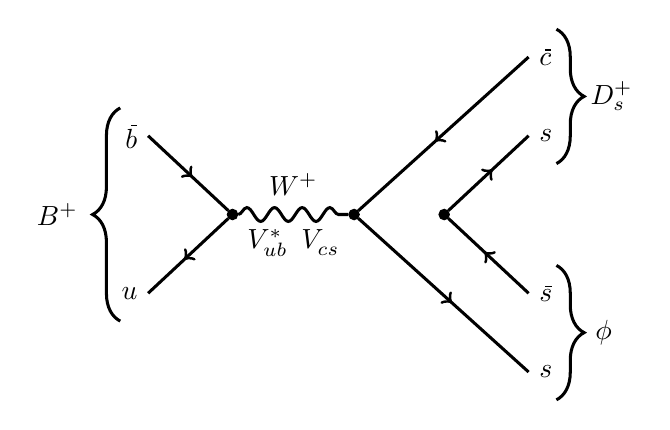
\begin{tikzpicture}[node distance=1cm and 1cm,line width=1.1pt]
  \coordinate[] (i1);
  \coordinate[below=1 of i1,label=left:\bquarkbar] (i2);
  \coordinate[below=2 of i1] (i3);
  \coordinate[below=3 of i1,label=left:\uquark] (i4);
  \coordinate[below=4 of i1] (i5);
  \coordinate[vertex,right=1 of i3,label=below right:$V_{ub}^*$] (v1);
  \coordinate[vertex,right=1.4 of v1,label=below left:$V_{cs}^{}$] (v2);
  \coordinate[vertex,right=1 of v2] (v3);
  \coordinate[right=1 of v3] (o3);
  \coordinate[above=2 of o3,label=right:\cquarkbar] (o1);
  \coordinate[above=1 of o3,label=right:\squark] (o2);
  \coordinate[below=1 of o3,label=right:\squarkbar] (o4);
  \coordinate[below=2 of o3,label=right:\squark] (o5);
  \draw[fermion] (i2) -- (v1);
  \draw[fermion] (v1) -- (i4);
  \draw[fermion] (o1) -- (v2);
  \draw[fermion] (v2) -- (o5);
  \draw[fermion] (o4) -- (v3);
  \draw[fermion] (v3) -- (o2);
  \draw[photon] (v1) -- (v2) node[midway,above=0.1] {$W^+$};
  \coordinate[above left=0.5 of i2] (bi1);
  \coordinate[below left=0.5 of i4] (bi2);
  \coordinate[above right=0.5 of o1] (bo1);
  \coordinate[below right=0.5 of o2] (bo2);
  \coordinate[above right=0.5 of o4] (bo3);
  \coordinate[below right=0.5 of o5] (bo4);
  \draw [decorate,decoration={brace,amplitude=10pt},xshift=4pt,yshift=0pt]
  (bi2) -- (bi1) node [black,midway,xshift=-0.8cm] {$\Bp$};
  \draw [decorate,decoration={brace,amplitude=10pt},xshift=4pt,yshift=0pt]
  (bo1) -- (bo2) node [black,midway,xshift=0.7cm] {$\Dsp$};
  \draw [decorate,decoration={brace,amplitude=10pt},xshift=4pt,yshift=0pt]
  (bo3) -- (bo4) node [black,midway,xshift=0.6cm] {$\phi$};
\end{tikzpicture}

%\newpage
%\pagebreak


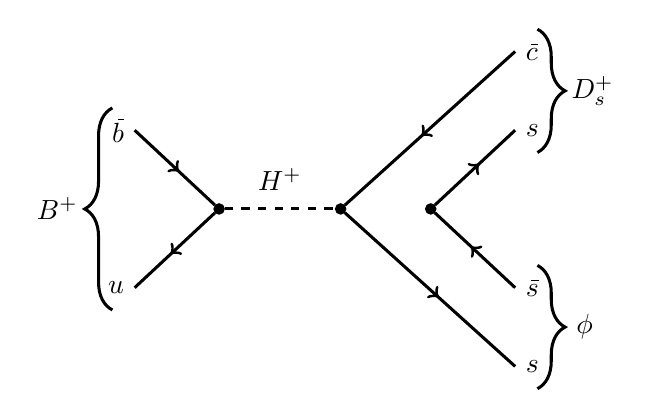
\begin{tikzpicture}[node distance=1cm and 1cm,line width=1.1pt]
  \coordinate[] (i1);
  \coordinate[below=1 of i1,label=left:\bquarkbar] (i2);
  \coordinate[below=2 of i1] (i3);
  \coordinate[below=3 of i1,label=left:\uquark] (i4);
  \coordinate[below=4 of i1] (i5);
  \coordinate[vertex,right=1 of i3] (v1);
  \coordinate[vertex,right=1.4 of v1] (v2);
  \coordinate[vertex,right=1 of v2] (v3);
  \coordinate[right=1 of v3] (o3);
  \coordinate[above=2 of o3,label=right:\cquarkbar] (o1);
  \coordinate[above=1 of o3,label=right:\squark] (o2);
  \coordinate[below=1 of o3,label=right:\squarkbar] (o4);
  \coordinate[below=2 of o3,label=right:\squark] (o5);
  \draw[fermion] (i2) -- (v1);
  \draw[fermion] (v1) -- (i4);
  \draw[fermion] (o1) -- (v2);
  \draw[fermion] (v2) -- (o5);
  \draw[fermion] (o4) -- (v3);
  \draw[fermion] (v3) -- (o2);
  \draw[higgs] (v1) -- (v2) node[midway,above=0.1] {$H^+$};
  \coordinate[above left=0.4 of i2] (bi1);
  \coordinate[below left=0.4 of i4] (bi2);
  \coordinate[above right=0.4 of o1] (bo1);
  \coordinate[below right=0.4 of o2] (bo2);
  \coordinate[above right=0.4 of o4] (bo3);
  \coordinate[below right=0.4 of o5] (bo4);
  \draw [decorate,decoration={brace,amplitude=10pt},xshift=4pt,yshift=0pt]
  (bi2) -- (bi1) node [black,midway,xshift=-0.7cm] {$\Bp$};
  \draw [decorate,decoration={brace,amplitude=10pt},xshift=4pt,yshift=0pt]
  (bo1) -- (bo2) node [black,midway,xshift=0.7cm] {$\Dsp$};
  \draw [decorate,decoration={brace,amplitude=10pt},xshift=4pt,yshift=0pt]
  (bo3) -- (bo4) node [black,midway,xshift=0.6cm] {$\phi$};
\end{tikzpicture}


%\begin{tikzpicture}[node distance=1cm and 1cm,line width=1.1pt]
  %%[line width=1.5 pt, scale=1.3]
  %\coordinate[label=left:\bquarkbar] (i1);
  %\coordinate[label=left:\uquark,below=5 of i1] (i2);
  %\coordinate[label=above left:$V_{tb}$,vertex,right=1.5 of i1] (v1);
  %\coordinate[label=above right:$V_{ts}$,vertex,right=2 of v1] (v2);
  %\coordinate[right=0.8 of v2] (d2);
  %\coordinate[left=0.3 of v2] (d3);
  %\coordinate[vertex,below=1.5 of d2] (v3);
  %\coordinate[vertex,below=3.5 of d2] (v4);
  %\coordinate[vertex,above=0.7 of d3] (v5);
  %\coordinate[vertex,above=1.5 of d2] (v6);
  %\coordinate[label=right:\squarkbar,right=1.8 of v2] (o1);
  %\coordinate[label=right:\uquark,below=1 of o1] (o2);
  %\coordinate[label=right:\uquarkbar,below=2 of o1] (o3);
  %\coordinate[label=right:\dquark,below=3 of o1] (o4);
  %\coordinate[label=right:\dquarkbar,below=4 of o1] (o5);
  %\coordinate[label=right:\uquark,below=5 of o1] (o6);
  %\coordinate[label=right:\mun,above=1 of o1] (o7);
  %\coordinate[label=right:\mup,above=2 of o1] (o8);
  %\draw[antifermion] (v1) arc (180:0:1.05) ++(-1.3,1.3) node[left] {\tquarkbar};
  %\draw[photonloop] (v2) arc (0:-180:1.05) ++(1.5,-0.7) node[left] {$W^+$};
  %\draw[antifermion] (i1) -- (v1);
  %\draw[fermion] (i2) -- (o6);
  %\draw[antifermion] (v2) -- (o1);
  %\draw[fermion] (v3) -- (o2);
  %\draw[antifermion] (v3) -- (o3);
  %\draw[fermion] (v4) -- (o4);
  %\draw[antifermion] (v4) -- (o5);
  %\draw[photon] (v6) -- (v5);
  %\draw[fermion] (v6) -- (o7);
  %\draw[antifermion] (v6) -- (o8);
  %\coordinate[above left=0.5 of i1] (bi1);
  %\coordinate[below left=0.5 of i2] (bi2);
  %\coordinate[above right=0.5 of o1] (bo1);
  %\coordinate[below right=0.5 of o2] (bo2);
  %\coordinate[above right=0.5 of o3] (bo3);
  %\coordinate[below right=0.5 of o4] (bo4);
  %\coordinate[above right=0.5 of o5] (bo5);
  %\coordinate[below right=0.5 of o6] (bo6);
  %\draw [decorate,decoration={brace,amplitude=10pt},xshift=4pt,yshift=0pt]
  %(bi2) -- (bi1) node [black,midway,xshift=-0.7cm] {$B^+$};
  %\draw [decorate,decoration={brace,amplitude=10pt},xshift=4pt,yshift=0pt]
  %(bo1) -- (bo2) node [black,midway,xshift=0.7cm] {$K^+$};
  %\draw [decorate,decoration={brace,amplitude=10pt},xshift=4pt,yshift=0pt]
  %(bo3) -- (bo4) node [black,midway,xshift=0.7cm] {$\pi^-$};
  %\draw [decorate,decoration={brace,amplitude=10pt},xshift=4pt,yshift=0pt]
  %(bo5) -- (bo6) node [black,midway,xshift=0.7cm] {$\pi^+$};
%\end{tikzpicture}


%\begin{tikzpicture}[node distance=1cm and 1cm,line width=1.1pt]
  %\coordinate[label=left:\bquarkbar] (i1);
  %\coordinate[label=left:\uquark,below=3.0 of i1] (i2);
  %\coordinate[label=above left:$V_{tb}$,vertex,right=1.5 of i1] (v1);
  %\coordinate[label=above right:$V_{ts}$,vertex,right=2 of v1] (v2);
  %\coordinate[right=0.8 of v2] (d2);
  %\coordinate[left=0.3 of v2] (d3);
  %\coordinate[vertex,below=1.5 of d2] (v3);
  %\coordinate[vertex,above=0.7 of d3] (v5);
  %\coordinate[vertex,above=1.5 of d2] (v6);
  %\coordinate[label=right:\squarkbar,right=1.8 of v2] (o1);
  %\coordinate[label=right:\squark,below=1 of o1] (o2);
  %\coordinate[label=right:\squarkbar,below=2 of o1] (o3);
  %\coordinate[label=right:\uquark,below=3 of o1] (o4);
  %\coordinate[label=right:\mun,above=1 of o1] (o7);
  %\coordinate[label=right:\mup,above=2 of o1] (o8);
  %\draw[antifermion] (v1) arc (180:0:1.05) ++(-1.3,1.3) node[left] {\tquarkbar};
  %\draw[photonloop] (v2) arc (0:-180:1.05) ++(1.5,-0.7) node[left] {$W^+$};
  %\draw[antifermion] (i1) -- (v1);
  %\draw[fermion] (i2) -- (o4);
  %\draw[antifermion] (v2) -- (o1);
  %\draw[fermion] (v3) -- (o2);
  %\draw[antifermion] (v3) -- (o3);
  %\draw[photon] (v6) -- (v5);
  %\draw[fermion] (v6) -- (o7);
  %\draw[antifermion] (v6) -- (o8);
  %\coordinate[above left=0.5 of i1] (bi1);
  %\coordinate[below left=0.5 of i2] (bi2);
  %\coordinate[above right=0.5 of o1] (bo1);
  %\coordinate[below right=0.5 of o2] (bo2);
  %\coordinate[above right=0.5 of o3] (bo3);
  %\coordinate[below right=0.5 of o4] (bo4);
  %\draw [decorate,decoration={brace,amplitude=10pt},xshift=4pt,yshift=0pt]
  %(bi2) -- (bi1) node [black,midway,xshift=-0.7cm] {$B^+$};
  %\draw [decorate,decoration={brace,amplitude=10pt},xshift=4pt,yshift=0pt]
  %(bo1) -- (bo2) node [black,midway,xshift=0.6cm] {$\phi$};
  %\draw [decorate,decoration={brace,amplitude=10pt},xshift=4pt,yshift=0pt]
  %(bo3) -- (bo4) node [black,midway,xshift=0.7cm] {$K^+$};
%\end{tikzpicture}


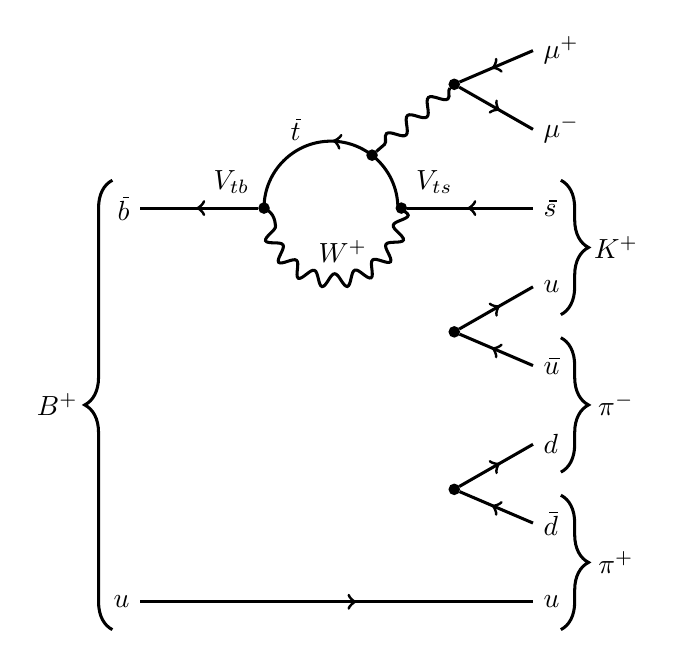
\begin{tikzpicture}[node distance=1cm and 1cm,line width=1.1pt]
  %[line width=1.5 pt, scale=1.3]
  \coordinate[label=left:\bquarkbar] (i1);
  \coordinate[label=left:\uquark,below=5 of i1] (i2);
  \coordinate[label=above left:$V_{tb}$,vertex,right=1.5 of i1] (v1);
  \coordinate[label=above right:$V_{ts}$,vertex,right=1.6 of v1] (v2);
  \coordinate[right=0.6 of v2] (d2);
  \coordinate[left=0.3 of v2] (d3);
  \coordinate[vertex,below=1.5 of d2] (v3);
  \coordinate[vertex,below=3.5 of d2] (v4);
  \coordinate[vertex,above=0.6 of d3] (v5);
  \coordinate[vertex,above=1.5 of d2] (v6);
  \coordinate[label=right:\squarkbar,right=1.6 of v2] (o1);
  \coordinate[label=right:\uquark,below=1 of o1] (o2);
  \coordinate[label=right:\uquarkbar,below=2 of o1] (o3);
  \coordinate[label=right:\dquark,below=3 of o1] (o4);
  \coordinate[label=right:\dquarkbar,below=4 of o1] (o5);
  \coordinate[label=right:\uquark,below=5 of o1] (o6);
  \coordinate[label=right:\mun,above=1 of o1] (o7);
  \coordinate[label=right:\mup,above=2 of o1] (o8);
  \draw[antifermion] (v1) arc (180:0:0.85) ++(-1.1,1.0) node[left] {\tquarkbar};
  \draw[photonloop] (v2) arc (0:-180:0.85) ++(1.4,-0.55) node[left] {$W^+$};
  \draw[antifermion] (i1) -- (v1);
  \draw[fermion] (i2) -- (o6);
  \draw[antifermion] (v2) -- (o1);
  \draw[fermion] (v3) -- (o2);
  \draw[antifermion] (v3) -- (o3);
  \draw[fermion] (v4) -- (o4);
  \draw[antifermion] (v4) -- (o5);
  \draw[photon] (v6) -- (v5);
  \draw[fermion] (v6) -- (o7);
  \draw[antifermion] (v6) -- (o8);
  \coordinate[above left=0.5 of i1] (bi1);
  \coordinate[below left=0.5 of i2] (bi2);
  \coordinate[above right=0.5 of o1] (bo1);
  \coordinate[below right=0.5 of o2] (bo2);
  \coordinate[above right=0.5 of o3] (bo3);
  \coordinate[below right=0.5 of o4] (bo4);
  \coordinate[above right=0.5 of o5] (bo5);
  \coordinate[below right=0.5 of o6] (bo6);
  \draw [decorate,decoration={brace,amplitude=10pt},xshift=4pt,yshift=0pt]
  (bi2) -- (bi1) node [black,midway,xshift=-0.7cm] {$B^+$};
  \draw [decorate,decoration={brace,amplitude=10pt},xshift=4pt,yshift=0pt]
  (bo1) -- (bo2) node [black,midway,xshift=0.7cm] {$K^+$};
  \draw [decorate,decoration={brace,amplitude=10pt},xshift=4pt,yshift=0pt]
  (bo3) -- (bo4) node [black,midway,xshift=0.7cm] {$\pi^-$};
  \draw [decorate,decoration={brace,amplitude=10pt},xshift=4pt,yshift=0pt]
  (bo5) -- (bo6) node [black,midway,xshift=0.7cm] {$\pi^+$};
\end{tikzpicture}


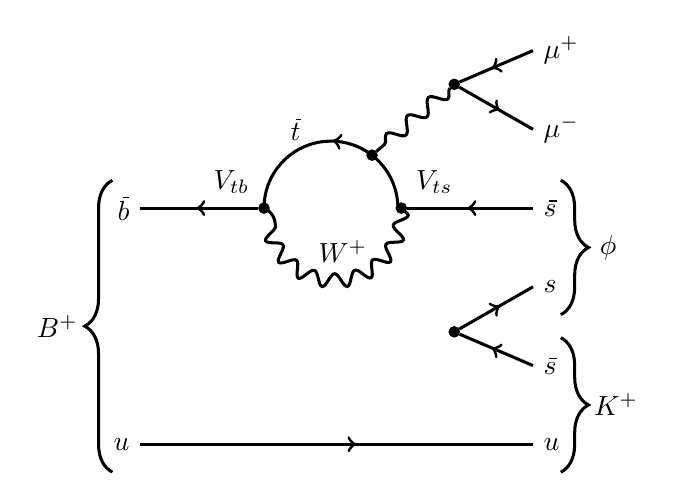
\begin{tikzpicture}[node distance=1cm and 1cm,line width=1.1pt]
  %[line width=1.5 pt, scale=1.3]
  \coordinate[label=left:\bquarkbar] (i1);
  \coordinate[label=left:\uquark,below=3 of i1] (i2);
  \coordinate[label=above left:$V_{tb}$,vertex,right=1.5 of i1] (v1);
  \coordinate[label=above right:$V_{ts}$,vertex,right=1.6 of v1] (v2);
  \coordinate[right=0.6 of v2] (d2);
  \coordinate[left=0.3 of v2] (d3);
  \coordinate[vertex,below=1.5 of d2] (v3);
  \coordinate[vertex,above=0.6 of d3] (v5);
  \coordinate[vertex,above=1.5 of d2] (v6);
  \coordinate[label=right:\squarkbar,right=1.6 of v2] (o1);
  \coordinate[label=right:\squark,below=1 of o1] (o2);
  \coordinate[label=right:\squarkbar,below=2 of o1] (o3);
  \coordinate[label=right:\uquark,below=3 of o1] (o4);
  \coordinate[label=right:\mun,above=1 of o1] (o7);
  \coordinate[label=right:\mup,above=2 of o1] (o8);
  \draw[antifermion] (v1) arc (180:0:0.85) ++(-1.1,1.0) node[left] {\tquarkbar};
  \draw[photonloop] (v2) arc (0:-180:0.85) ++(1.4,-0.55) node[left] {$W^+$};
  \draw[antifermion] (i1) -- (v1);
  \draw[fermion] (i2) -- (o4);
  \draw[antifermion] (v2) -- (o1);
  \draw[fermion] (v3) -- (o2);
  \draw[antifermion] (v3) -- (o3);
  \draw[photon] (v6) -- (v5);
  \draw[fermion] (v6) -- (o7);
  \draw[antifermion] (v6) -- (o8);
  \coordinate[above left=0.5 of i1] (bi1);
  \coordinate[below left=0.5 of i2] (bi2);
  \coordinate[above right=0.5 of o1] (bo1);
  \coordinate[below right=0.5 of o2] (bo2);
  \coordinate[above right=0.5 of o3] (bo3);
  \coordinate[below right=0.5 of o4] (bo4);
  \draw [decorate,decoration={brace,amplitude=10pt},xshift=4pt,yshift=0pt]
  (bi2) -- (bi1) node [black,midway,xshift=-0.7cm] {$B^+$};
  \draw [decorate,decoration={brace,amplitude=10pt},xshift=4pt,yshift=0pt]
  (bo1) -- (bo2) node [black,midway,xshift=0.6cm] {$\phi$};
  \draw [decorate,decoration={brace,amplitude=10pt},xshift=4pt,yshift=0pt]
  (bo3) -- (bo4) node [black,midway,xshift=0.7cm] {$K^+$};
\end{tikzpicture}


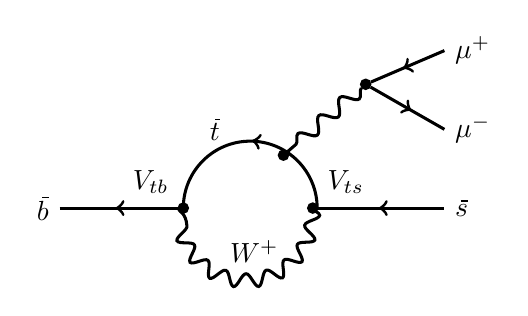
\begin{tikzpicture}[node distance=1cm and 1cm,line width=1.1pt]
  \coordinate[label=left:\bquarkbar] (i1);
  \coordinate[label=above left:$V_{tb}$,vertex,right=1.5 of i1] (v1);
  \coordinate[label=above right:$V_{ts}$,vertex,right=1.5 of v1] (v2);
  \coordinate[right=0.6 of v2] (d2);
  \coordinate[left=0.3 of v2] (d3);
  \coordinate[vertex,above=0.6 of d3] (v5);
  \coordinate[vertex,above=1.5 of d2] (v6);
  \coordinate[label=right:\squarkbar,right=1.6 of v2] (o1);
  \coordinate[label=right:\mun,above=1 of o1] (o7);
  \coordinate[label=right:\mup,above=2 of o1] (o8);
  \draw[antifermion] (v1) arc (180:0:0.85) ++(-1.1,1.0) node[left] {\tquarkbar};
  \draw[photonloop] (v2) arc (0:-180:0.85) ++(1.4,-0.55) node[left] {$W^+$};
  \draw[antifermion] (i1) -- (v1);
  \draw[antifermion] (v2) -- (o1);
  \draw[photon] (v6) -- (v5);
  \draw[fermion] (v6) -- (o7);
  \draw[antifermion] (v6) -- (o8);
\end{tikzpicture}


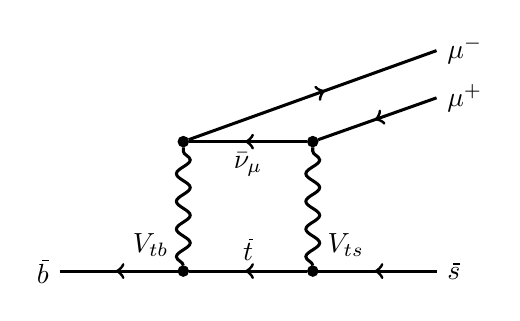
\begin{tikzpicture}[node distance=1cm and 1cm,line width=1.1pt]
  \coordinate[label=left:\bquarkbar] (i1);
  \coordinate[label=above left:$V_{tb}$,vertex,right=1.5 of i1] (v1);
  \coordinate[vertex,above=1.5 of v1] (v2);
  \coordinate[label=above right:$V_{ts}$,vertex,right=1.5 of v1] (v3);
  \coordinate[vertex,right=1.5 of v2] (v4);
  \coordinate[label=right:\squarkbar,right=1.5 of v3] (o1);
  \coordinate[label=right:\mup,above=2.2 of o1] (o2);
  \coordinate[label=right:\mun,above=2.8 of o1] (o3);
  \draw[antifermion] (i1) -- (v1);
  \draw[antifermion] (v1) -- (v3) node[midway,above] {$\tquarkbar$};
  \draw[antifermion] (v3) -- (o1);
  \draw[antifermion] (v2) -- (v4) node[midway,below] {$\bar{\nu}_\mu$};
  \draw[photon] (v1) -- (v2);
  \draw[photon] (v3) -- (v4);
  \draw[fermion] (v2) -- (o3);
  \draw[antifermion] (v4) -- (o2);
\end{tikzpicture}


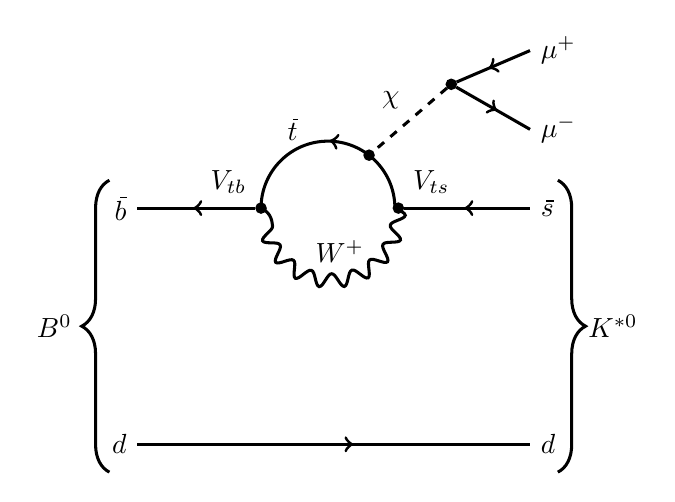
\begin{tikzpicture}[node distance=1cm and 1cm,line width=1.1pt]
  %[line width=1.5 pt, scale=1.3]
  \coordinate[label=left:\bquarkbar] (i1);
  \coordinate[label=left:\dquark,below=3 of i1] (i2);
  \coordinate[label=above left:$V_{tb}$,vertex,right=1.5 of i1] (v1);
  \coordinate[label=above right:$V_{ts}$,vertex,right=1.6 of v1] (v2);
  \coordinate[right=0.6 of v2] (d2);
  \coordinate[left=0.3 of v2] (d3);
  %\coordinate[vertex,below=1.5 of d2] (v3);
  \coordinate[vertex,above=0.6 of d3] (v5);
  \coordinate[vertex,above=1.5 of d2] (v6);
  \coordinate[label=right:\squarkbar,right=1.6 of v2] (o1);
  %\coordinate[label=right:\squark,below=1 of o1] (o2);
  %\coordinate[label=right:\squarkbar,below=2 of o1] (o3);
  \coordinate[label=right:\dquark,below=3 of o1] (o2);
  \coordinate[label=right:\mun,above=1 of o1] (o7);
  \coordinate[label=right:\mup,above=2 of o1] (o8);
  \draw[antifermion] (v1) arc (180:0:0.85) ++(-1.1,1.0) node[left] {\tquarkbar};
  \draw[photonloop] (v2) arc (0:-180:0.85) ++(1.4,-0.55) node[left] {$W^+$};
  \draw[antifermion] (i1) -- (v1);
  \draw[fermion] (i2) -- (o2);
  \draw[antifermion] (v2) -- (o1);
  %\draw[fermion] (v3) -- (o2);
  %\draw[antifermion] (v3) -- (o3);
  \draw[higgs] (v6) -- (v5) node[midway,above left] {$\chi$};
  \draw[fermion] (v6) -- (o7);
  \draw[antifermion] (v6) -- (o8);
  \coordinate[above left=0.5 of i1] (bi1);
  \coordinate[below left=0.5 of i2] (bi2);
  \coordinate[above right=0.5 of o1] (bo1);
  \coordinate[below right=0.5 of o2] (bo2);
  %\coordinate[above right=0.5 of o3] (bo3);
  %\coordinate[below right=0.5 of o4] (bo4);
  \draw [decorate,decoration={brace,amplitude=10pt},xshift=4pt,yshift=0pt]
  (bi2) -- (bi1) node [black,midway,xshift=-0.7cm] {$B^0$};
  \draw [decorate,decoration={brace,amplitude=10pt},xshift=4pt,yshift=0pt]
  (bo1) -- (bo2) node [black,midway,xshift=0.7cm] {$\Kstarz$};
\end{tikzpicture}


%\begin{tikzpicture}[node distance=1cm and 1cm,line width=1.1pt]
  %%[line width=1.5 pt, scale=1.3]
  %\coordinate[vertex, label=left:\bquarkbar] (i0);
  %\coordinate[vertex, below=2.5 of i0, label=left:\dquark] (i1);
  %\coordinate[right=2 of i1] (d1);
  %\coordinate[right=2 of d1] (d2);
  %\coordinate[vertex, right=2 of d2, label=right:\dquark] (o3);
  %\coordinate[vertex, above=1 of o3, label=right:$\cquark/\uquark$] (o2);
  %\coordinate[vertex, above=2 of o3, label=right:\uquark] (o1);
  %\coordinate[vertex, above=3 of o3, label=right:\mun] (o0);
  %\coordinate[right=0.25 of o1] (d3);
  %\coordinate[right=0.25 of o3] (d4);
  %\coordinate[vertex, above=1.5 of d2, label=above:?$_2$] (v1);
  %\coordinate[vertex, above=2.5 of d1, label=above:?$_1$] (v0);
  %\draw[fermion] (v0) -- (i0);
  %\draw[fermion] (o0) -- (v0);
  %\draw[fermion] (v1) -- (o1);
  %\draw[fermion] (v1) -- (o2);
  %\draw[fermion] (i1) -- (o3);
  %\draw[higgs] (v0) -- (v1) node [midway,below left] {$+\tfrac43$};
  %\coordinate[above left=0.5 of i0] (bi0);
  %\coordinate[below left=0.5 of i1] (bi1);
  %\coordinate[above right=0.5 of d3] (bo0);
  %\coordinate[below right=0.5 of d4] (bo1);
  %\draw [decorate,decoration={brace,amplitude=10pt},xshift=4pt,yshift=0pt]
  %(bi1) -- (bi0) node [black,midway,xshift=-0.7cm] {$B^0$};
  %\draw [decorate,decoration={brace,amplitude=10pt},xshift=4pt,yshift=0pt]
  %(bo0) -- (bo1) node [black,midway,xshift=0.9cm] {$\Lc/p$};
%\end{tikzpicture}


%\begin{tikzpicture}[node distance=1cm and 1cm,line width=1.1pt]
\begin{tikzpicture} [line width=1.5 pt, scale=1.3]
  %[line/.style={-,shorten >=0.4cm,shorten <=0.4cm},thick]
  %%%%%%%
  % (rho,eta) = (0.131,0.345) * 5 = (0.655,1.725)
  % gamma = 68, alpha = 89, beta = 23
  %%%%%%%
  \coordinate[svertex,label=below:{$(0,0)$}] (gamma);
  \coordinate[] (gamma) ++(0:5) node (beta) [svertex,label=below:{$(1,0)$}] {};
  \coordinate[] (gamma) ++(68:1.845) node (alpha) [svertex,label=above:{$(\bar\rho,\bar\eta)$}] {};
  \path (gamma) ++(0:0.3) node (gammaarc0) [] {};
  \path (gamma) ++(68:0.3) node (gammaarc1) [] {};
  \path (alpha) ++(-23:0.3) node (alphaarc0) [] {};
  \path (alpha) ++(-112:0.3) node (alphaarc1) [] {};
  \path (beta) ++(180:0.6) node (betaarc0) [] {};
  \path (beta) ++(157:0.6) node (betaarc1) [] {};

  \path (gamma) ++(34:0.6) node (gammalabel) [] {$\gamma$};
  \path (alpha) ++(-68:0.6) node (alphalabel) [] {$\alpha$};
  \path (beta) ++(170:1.2) node (betalabel) [] {$\beta$};

  \draw (alphaarc1) arc (-112:-23:0.3);
  \draw (gammaarc0) arc (0:68:0.3);
  \draw (betaarc0) arc (180:157:0.6) [];

  \path (gamma) ++(25:3.3) node (gammaopposite) [] {
    \large
    $\left|\frac{V_{{td}}^{}V_{{tb}}^*}
    {V_{\kern-0.1em{cd}}^{}V_{\kern-0.1em{cb}}^*}\right|$
  };
  \path (beta) ++(170:5.5) node (betaopposite) [] {
    \large
    $\left|\frac{V_{\kern-0.1em{ud}}^{}V_{\kern-0.1em{ub}}^*}
    {V_{\kern-0.1em{cd}}^{}V_{\kern-0.1em{cb}}^*}\right|$
  };
  \draw [line cap=round] (alpha) -- (beta);
  \draw [line cap=round] (alpha) -- (gamma);
  \draw [line cap=round] (gamma) -- (beta);


  %\draw (gamma) ++(-0.09825,-0.25875) arc (-88:-40:0.5);
  %\path [black,line,line,out=135,in=225] (alpha) edge (gamma);
  %\draw (gamma) ++(-0.09825,-0.25875) arc (89:-68:1);
  %\draw[fermion] (o0) -- (v0);
  %\draw[fermion] (v1) -- (o1);
  %\draw[fermion] (v1) -- (o2);
  %\draw[fermion] (i1) -- (o3);
  %\draw[higgs] (v0) -- (v1) node [midway,below left] {$+\tfrac43$};
  %\coordinate[above left=0.5 of i0] (bi0);
  %\coordinate[below left=0.5 of i1] (bi1);
  %\coordinate[above right=0.5 of d3] (bo0);
  %\coordinate[below right=0.5 of d4] (bo1);
  %\draw [decorate,decoration={brace,amplitude=10pt},xshift=4pt,yshift=0pt]
  %(bi1) -- (bi0) node [black,midway,xshift=-0.7cm] {$B^0$};
  %\draw [decorate,decoration={brace,amplitude=10pt},xshift=4pt,yshift=0pt]
  %(bo0) -- (bo1) node [black,midway,xshift=0.9cm] {$\Lc/p$};
\end{tikzpicture}

%\begin{tikzpicture}[line/.style={<->,shorten >=0.4cm,shorten <=0.4cm},thick]
  %%\node[anchor=south west,inner sep=0] at (0,0) {\includegraphics{hnRDQ.png}};
  %\coordinate (G) ;
  %\node (R) [circle,draw,inner sep=0pt,minimum width=1.5cm] at (6.4,3.9) {};
  %\node (B) [circle,draw,inner sep=0pt,minimum width=1cm] at (2.1,1.7) {};
  %\path [green,line,bend left] (G) edge (R);
  %\path [red,bend left,line]   (R) edge (B);
  %\path [black,line,out=135,in=225] (B) edge (G); % you can control the bend by manually specifying in=<angle> and out=<angle> options
%\end{tikzpicture}


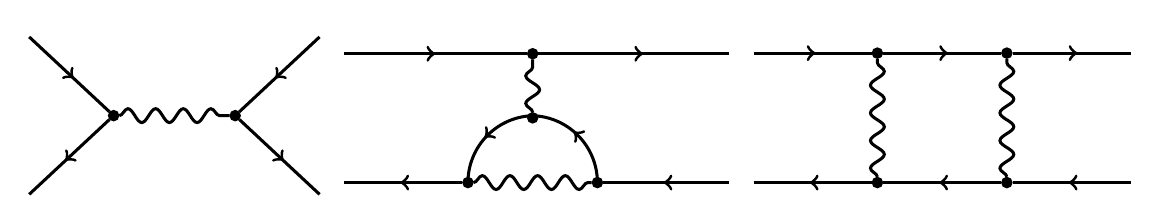
\begin{tikzpicture}[node distance=1cm and 1cm,line width=1.1pt]
  \coordinate[] (treei1);


  \coordinate[below=1 of treei1] (treei2);
  \coordinate[below=2 of treei1] (treei3);
  \coordinate[below=3 of treei1] (treei4);
  \coordinate[below=4 of treei1] (treei5);
  \coordinate[vertex,right=1 of treei3] (treev1);
  \coordinate[vertex,right=1.4 of treev1] (treev2);
  \coordinate[right=1 of treev2] (treev3);
  \coordinate[above=1 of treev3] (treeo1);
  \coordinate[below=1 of treev3] (treeo2);
  \draw[fermion] (treei2) -- (treev1);
  \draw[fermion] (treev1) -- (treei4);
  \draw[fermion] (treeo1) -- (treev2);
  \draw[fermion] (treev2) -- (treeo2);
  \draw[photon] (treev1) -- (treev2) node[midway,above=0.1] {};

  \coordinate[right=4 of treei4] (dummy1);
  \coordinate[above=0.15 of dummy1] (pengi1);

  \coordinate[vertex,right=1.5 of pengi1] (pengv1);
  \coordinate[vertex,right=1.5 of pengv1] (pengv2);
  \coordinate[right=0.75 of pengv1] (pengv3);
  \coordinate[vertex,above=0.75 of pengv3] (pengv4);
  \coordinate[vertex,above=0.67 of pengv4] (pengv5);
  \coordinate[left=2.32 of pengv5] (pengi2);
  \coordinate[right=2.42 of pengv5] (pengo2);
  \coordinate[right=1.6 of pengv2] (pengo1);
  \draw[antifermion] (pengv1) arc (180:90:0.85) ++(-1.1,1.0) node[left] {};
  \draw[fermion] (pengv2) arc (0:90:0.85) ++(-1.1,1.0) node[left] {};
  \draw[photon] (pengv1) -- (pengv2);
  \draw[photon] (pengv4) -- (pengv5);
  \draw[antifermion] (pengi1) -- (pengv1);
  \draw[antifermion] (pengv2) -- (pengo1);
  \draw[antifermion] (pengv5) -- (pengi2);
  \draw[fermion] (pengv5) -- (pengo2);

  \coordinate[right=5.2 of dummy1] (dummy2);
  \coordinate[above=0.15 of dummy2] (boxi1);
  \coordinate[vertex,right=1.5 of boxi1] (boxv1);
  \coordinate[vertex,above=1.5 of boxv1] (boxv2);
  \coordinate[vertex,right=1.5 of boxv1] (boxv3);
  \coordinate[vertex,right=1.5 of boxv2] (boxv4);
  \coordinate[left=1.5 of boxv2] (boxi2);
  \coordinate[right=1.5 of boxv3] (boxo1);
  \coordinate[right=1.5 of boxv4] (boxo2);
  \draw[antifermion] (boxi1) -- (boxv1);
  \draw[antifermion] (boxv1) -- (boxv3);
  \draw[antifermion] (boxv3) -- (boxo1);
  \draw[fermion] (boxv2) -- (boxv4);
  \draw[photon] (boxv1) -- (boxv2);
  \draw[photon] (boxv3) -- (boxv4);
  \draw[antifermion] (boxv2) -- (boxi2);
  \draw[fermion] (boxv4) -- (boxo2);

\end{tikzpicture}







\end{document}
